\documentclass{article}

\usepackage{geometry}
\geometry{a4paper, scale=0.8}

\usepackage{graphicx}

\usepackage{ctex}

\title{ISOA Progress Report}
\author{Group "200"\\YiDai 2017013562\\ZhaohengLi 2017050025}

\begin{document}
\maketitle
\section{项目介绍}
我们以疫情部分的舆论方面为核心,提取舆论主题,结合时间线展示群众的关注点变化,对访问者提供舆论谣言判断服务。同时我们也注意到,信息服务平台如果缺失一方面的关键信息很容易丧失吸引力,我们还会实现政府的相关措施发布、并实现确诊数据展示。

主要实现目标如下:
\begin{itemize}
	\item{\textbf{疫情展示}} 主要包括疫情确诊地图、详细数字和相关新闻或政策的时间线。
	\item{\textbf{舆情关注展示}} 对舆情进行主题提取,结合时间线展示群众的关注点变化
	\item{\textbf{虚假新闻/谣言判断及搜索}} 用户输入文本,对文本进行分析,为用户提供相关已证实谣言或者相关新闻,并给出用户输入文本为谣言的概率。
\end{itemize}

周计划制定如下:
\begin{figure}[htb]
\centering
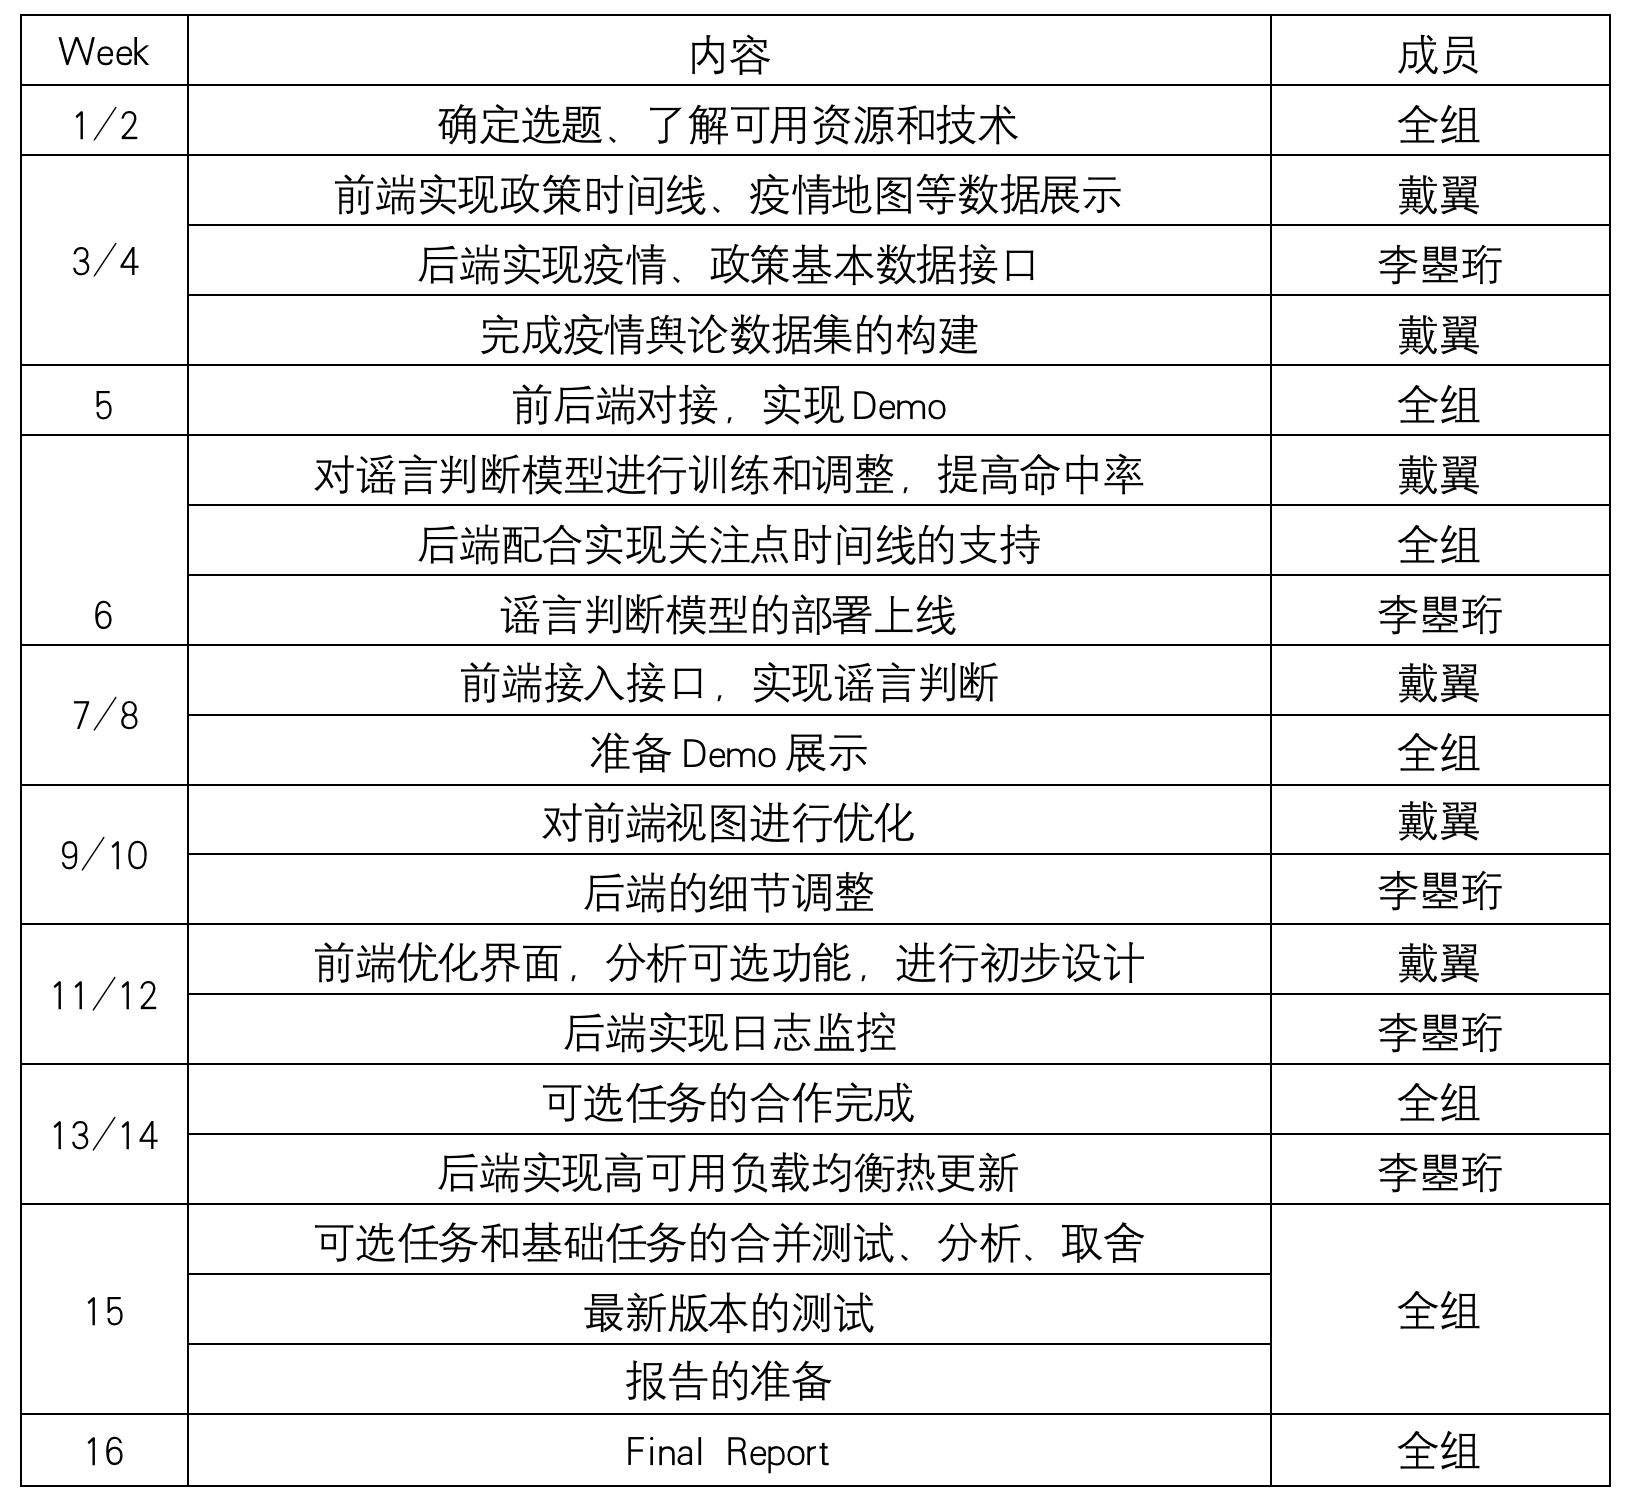
\includegraphics[width=0.5\textwidth]{pic1.png}
\end{figure}

\section{后端部分进展}
\subsection{后端架构}
为了降低项目的耦合性,后端使用Web应用程序框架Flask进行实现和封装。通过网络接口,可以使前端获得所需要的数据而不用关心后端的实现方法。

我们的项目所提供的信息时效性很强,为了提高服务的稳定性和实效性,我们使用了MySQL数据库存储收集到的数据,并且已经部署了数据定时更新的工作。

\subsection{数据处理}
目前收集到并整理出的数据有
\begin{itemize}
	\item{\textbf{疫情数据}} 自2020年1月22日至今,中国所有省份、地区或直辖市及世界其他国家的所有疫情信息变化的时间序列数据(精确到市),能够追溯确诊/疑似感染/治愈/死亡人数的时间序列。疫情数据目前已经完成整理,并提供给前端供疫情可视化部分使用;
	\item{\textbf{新闻数据}} 自病发开始各个省份、地区或直辖市及世界其他国家关于疫情所发布的新闻。新闻数据目前已经按照发布时间,发布地点进行了分类整理。
	\item{\textbf{谣言数据}} 与疫情有关的谣言以及丁香园的辟谣信息。谣言数据目前已经按照“谣言”、“权威数据”和“未证实”的标签对内容进行了分类处理。
\end{itemize}

\subsection{接口处理}

目前后端获得的数据已经比较完善,因此计划中的接口已经全部实现。下面为列举的几个主要接口:
\begin{itemize}
	\item{\textbf{route('/getDataSummary')}} 提供后端数据收集情况概览 
	\item{\textbf{route('/getTimeData')}} 根据时间参数提供全国当天的疫情发展数据
	\item{\textbf{route('/getDataPos')}} 根据地区参数提供该地区的疫情历史发展数据
	\item{\textbf{route('/getNewsData')}} 根据地区和时间参数获取某个地区某个时刻的新闻列表
	\item{\textbf{route('/getRumorData')}} 根据内容类型参数提供该类型的谣言数据
	\item{\textbf{route('/getMap')}} 提供疫情分布的地图数据
\end{itemize}

\subsection{遇到的问题}
目前后端进展比较顺利,没有遇到较大的问题,完成了预期的计划内容。

\subsection{未来计划}
接下来的工作是我们的项目的核心,涉及到“提取舆论主题”、“结合时间线展示群众的关注点变化”以及“谣言判断”等相关工作,要使用神经网络模型对我们收集到的数据进行主题提取和内容分类等一系列操作。

对于后端数据部分,原来制定的计划不会有大的改变,所以接下来几周的重点会放在“舆论数据的收集和进一步的整理”以及“神经网络模型判断谣言“两部分。



\section{前端部分进展}
目前疫情信息平台已经实现前后端基本端口的对接,已经完成在阿里云服务器上的自动挂载,可以通过外部IP访问、并查看实时疫情信息。
\subsection{前端架构}
前端使用Vue.js框架,实现了疫情实时数据(包括舆情)、疫情新闻两个主页面,为了将页面篇幅利用率合理化,我们利用栏目切换展示疫情数据的几个角度:
\begin{itemize}
	\item 全国实时疫情
	\item 全国各省疫情回放
	\item 省实时疫情
	\item 各省各项数据曲线分析 
	\item 舆情时间线分析
\end{itemize}
\begin{figure}[htb]
\centering
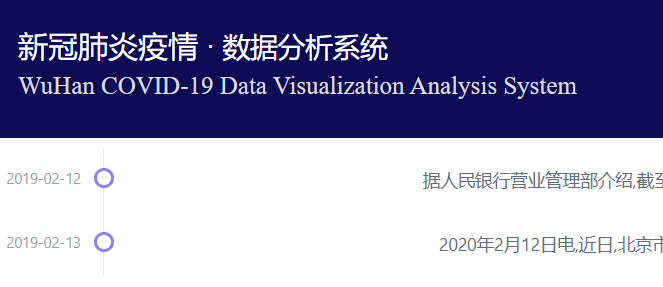
\includegraphics[width=0.8\textwidth]{pic2.png}
\end{figure}

\begin{figure}[htb]
\centering
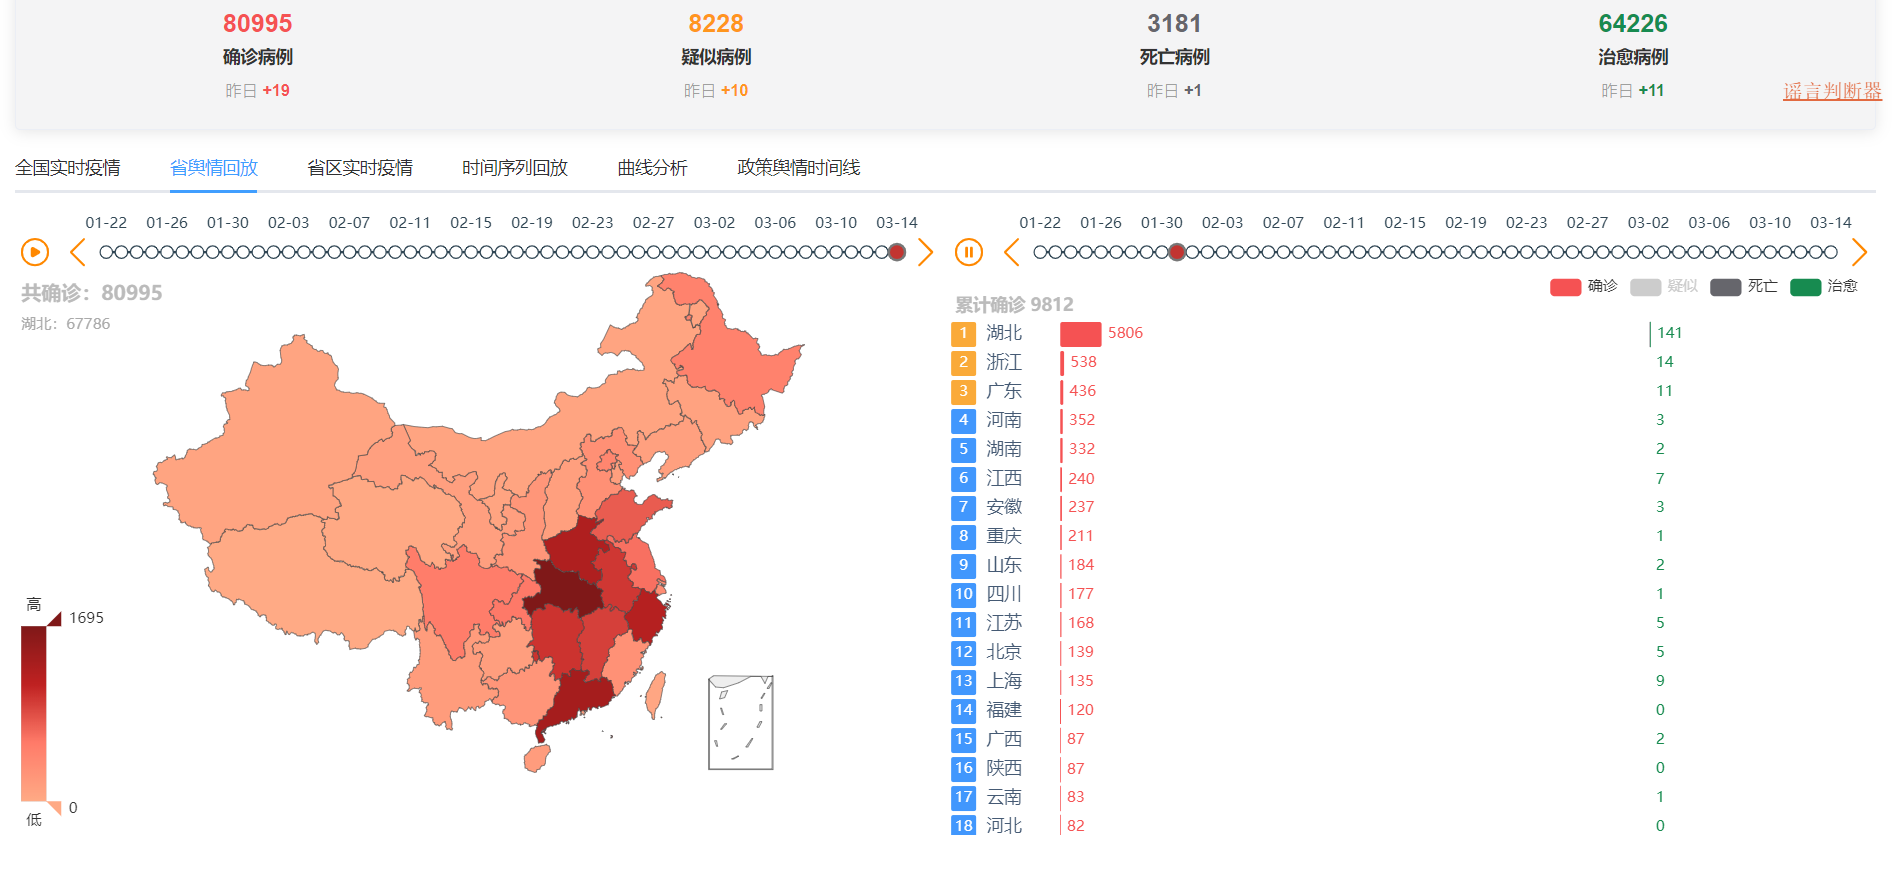
\includegraphics[width=0.8\textwidth]{pic3.png}
\end{figure}

依靠后端提供的地图和省区数据和Echarts的绘制功能,我们实现了在地图上点击即可切换地图、获取各地疫情的功能;依靠后端MySQL的长时间存储,结合前端的Timeline组件,实现了疫情、舆情的时间线回放。


\section{预测模型部分进展}
我们已经完成了疫情舆论数据集的构建,将丁香园提供的舆情加入传统的微博和twitter谣言语料库训练,并且结合Flask形成了外部服务接口,已经交给后端开始疫情数据提供、谣言判断两个模块的组合。

在网络结构上,我们借鉴已有的工作,用Transformer+卷积层的方式对文本进行语义信息提取,其在仅CPU的条件下运行速度较快。

\section{进展总结}
\subsection{遇到的问题}
目前而言,前后端进展比较顺利,没有遇到较大的问题,完成了预期的计划内容。

疫情舆论数据集构建面临的情况,主要是丁香园提供数据集的不充分、且在现有条件下进行人工标注不现实,所以我们采取了折中的方法,结合了已有的舆论数据集。

此外,在缺失传统谣言判断任务中的用户id情况下,模型测试正确率会有降低,所以我们采取的方案是在未来结合关键词提取等Non-Neural的方法,提高该功能的可靠性。

\subsection{未来计划}
接下来的工作是我们的项目的核心,涉及到“提取舆论主题”、“结合时间线展示群众的关注点变化”以及“谣言判断”等相关工作,要使用神经网络模型对我们收集到的数据进行主题提取和内容分类等一系列操作。

对于后端数据部分,原来制定的计划不会有大的改变,所以接下来几周的重点会放在“舆论数据的收集和进一步的整理”以及“神经网络模型判断谣言“两部分。
对于前端部分,需要对后端新加入的舆论数据提供进行对接,并完成神经网络模型判断谣言的前端界面。

整体而言,我们制定的Schedule不会发生太大改变,原本第五周仅用来对接和实现Demo,现在我们会利用第五周对接更多接口,提高初步上线Demo的质量、考虑域名等细节事宜。此外,我们原定第六周将谣言预测部署上线,现在我们将提早进行部署、效果(主要是用户体验)评估,以便后期完善。


\end{document}